\begin{pa} \label{PA:1.5}
One of the longest stretches of straight (and flat) road in North America can be found on the Great Plains in the state of North Dakota on state highway 46, which lies just south of the interstate highway I-94 and runs through the town of Gackle.  A car leaves town (at time $t = 0$) and heads east on highway 46; its position in miles from Gackle at time $t$ in minutes is given by the graph of the function in Figure~\ref{F:1.5.PA1}.  Three important points are labeled on the graph; where the curve looks linear, assume that it is indeed a straight line.
\begin{figure}[h]
\begin{center}
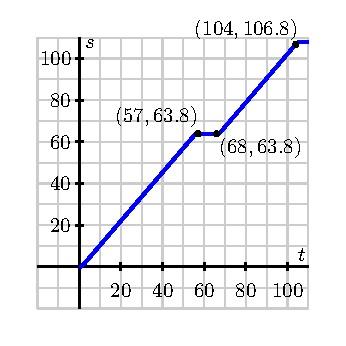
\includegraphics{figures/1_5_PA1.eps}
\caption{The graph of $y = s(t)$, the position of the car along highway 46, which tells its distance in miles from Gackle, ND, at time $t$ in minutes.} \label{F:1.5.PA1}
\end{center}
\end{figure}
\ba
	\item In everyday language, describe the behavior of the car over the provided time interval.  In particular, discuss what is happening on the time intervals $[57,68]$ and $[68,104]$.
	\item Find the slope of the line between the points $(57,63.8)$ and $(104,106.8)$.  What are the units on this slope?  What does the slope represent?
	\item Find the average rate of change of the car's position on the interval $[68,104]$.  Include units on your answer.
	\item Estimate the instantaneous rate of change of the car's position at the moment $t = 80$.  Write a sentence to explain your reasoning and the meaning of this value.
\ea
\end{pa} \afterpa

